\documentclass[../../main.tex]{subfiles}

\begin{document}

\subsection{WFC Variants and Applications}
\label{subsec:related_wfc_variants}

Since its introduction by Gumin~\citeonline{Gumin2016wfc}, Wave Function Collapse has been applied to many different domains and extended to overcome some of the limitations of the original algorithm.

\paragraph{Formalization and Different Strategies.}

Karth and Smith~\citebibliography{Karth2022a} provided a formal description of the WFC algorithm. They studied different strategies for cells and tiles selection, as well as the use of backtracking and global constraints. Their results showed that these choices can significantly affect both the generation process and the final output. In particular, they showed that the restart from scratch strategy used in Gumin's original implementation works well with simple local rules, but becomes less effective when global constraints are introduced. In such cases, the number of contradictions increases significantly, making backtracking essential.

\paragraph{Game Development.}

WFC has been widely used in game development for environment and level generation. Parker and Jones used it in \emph{Proc Skater 2016}~\citeonline{ParkerProcSkater} to generate unique skateboard parks. Stålberg used WFC in \emph{Bad North}~\citeonline{StalbergBadNorth} to generate 3D islands and in \emph{Townscaper}~\citeonline{StalbergTownscaper} to turn player clicks into coherent buildings. Kleineberg~\citeonline{KleinebergInfiniteCity} created \emph{Infinite City}, a game that generates a city as the player explores it. Examples are shown in \figref{fig:wfc_game_development}.

\begin{figure}[h]
    \centering

    \begin{subfigure}[b]{0.48\linewidth}
        \centering
        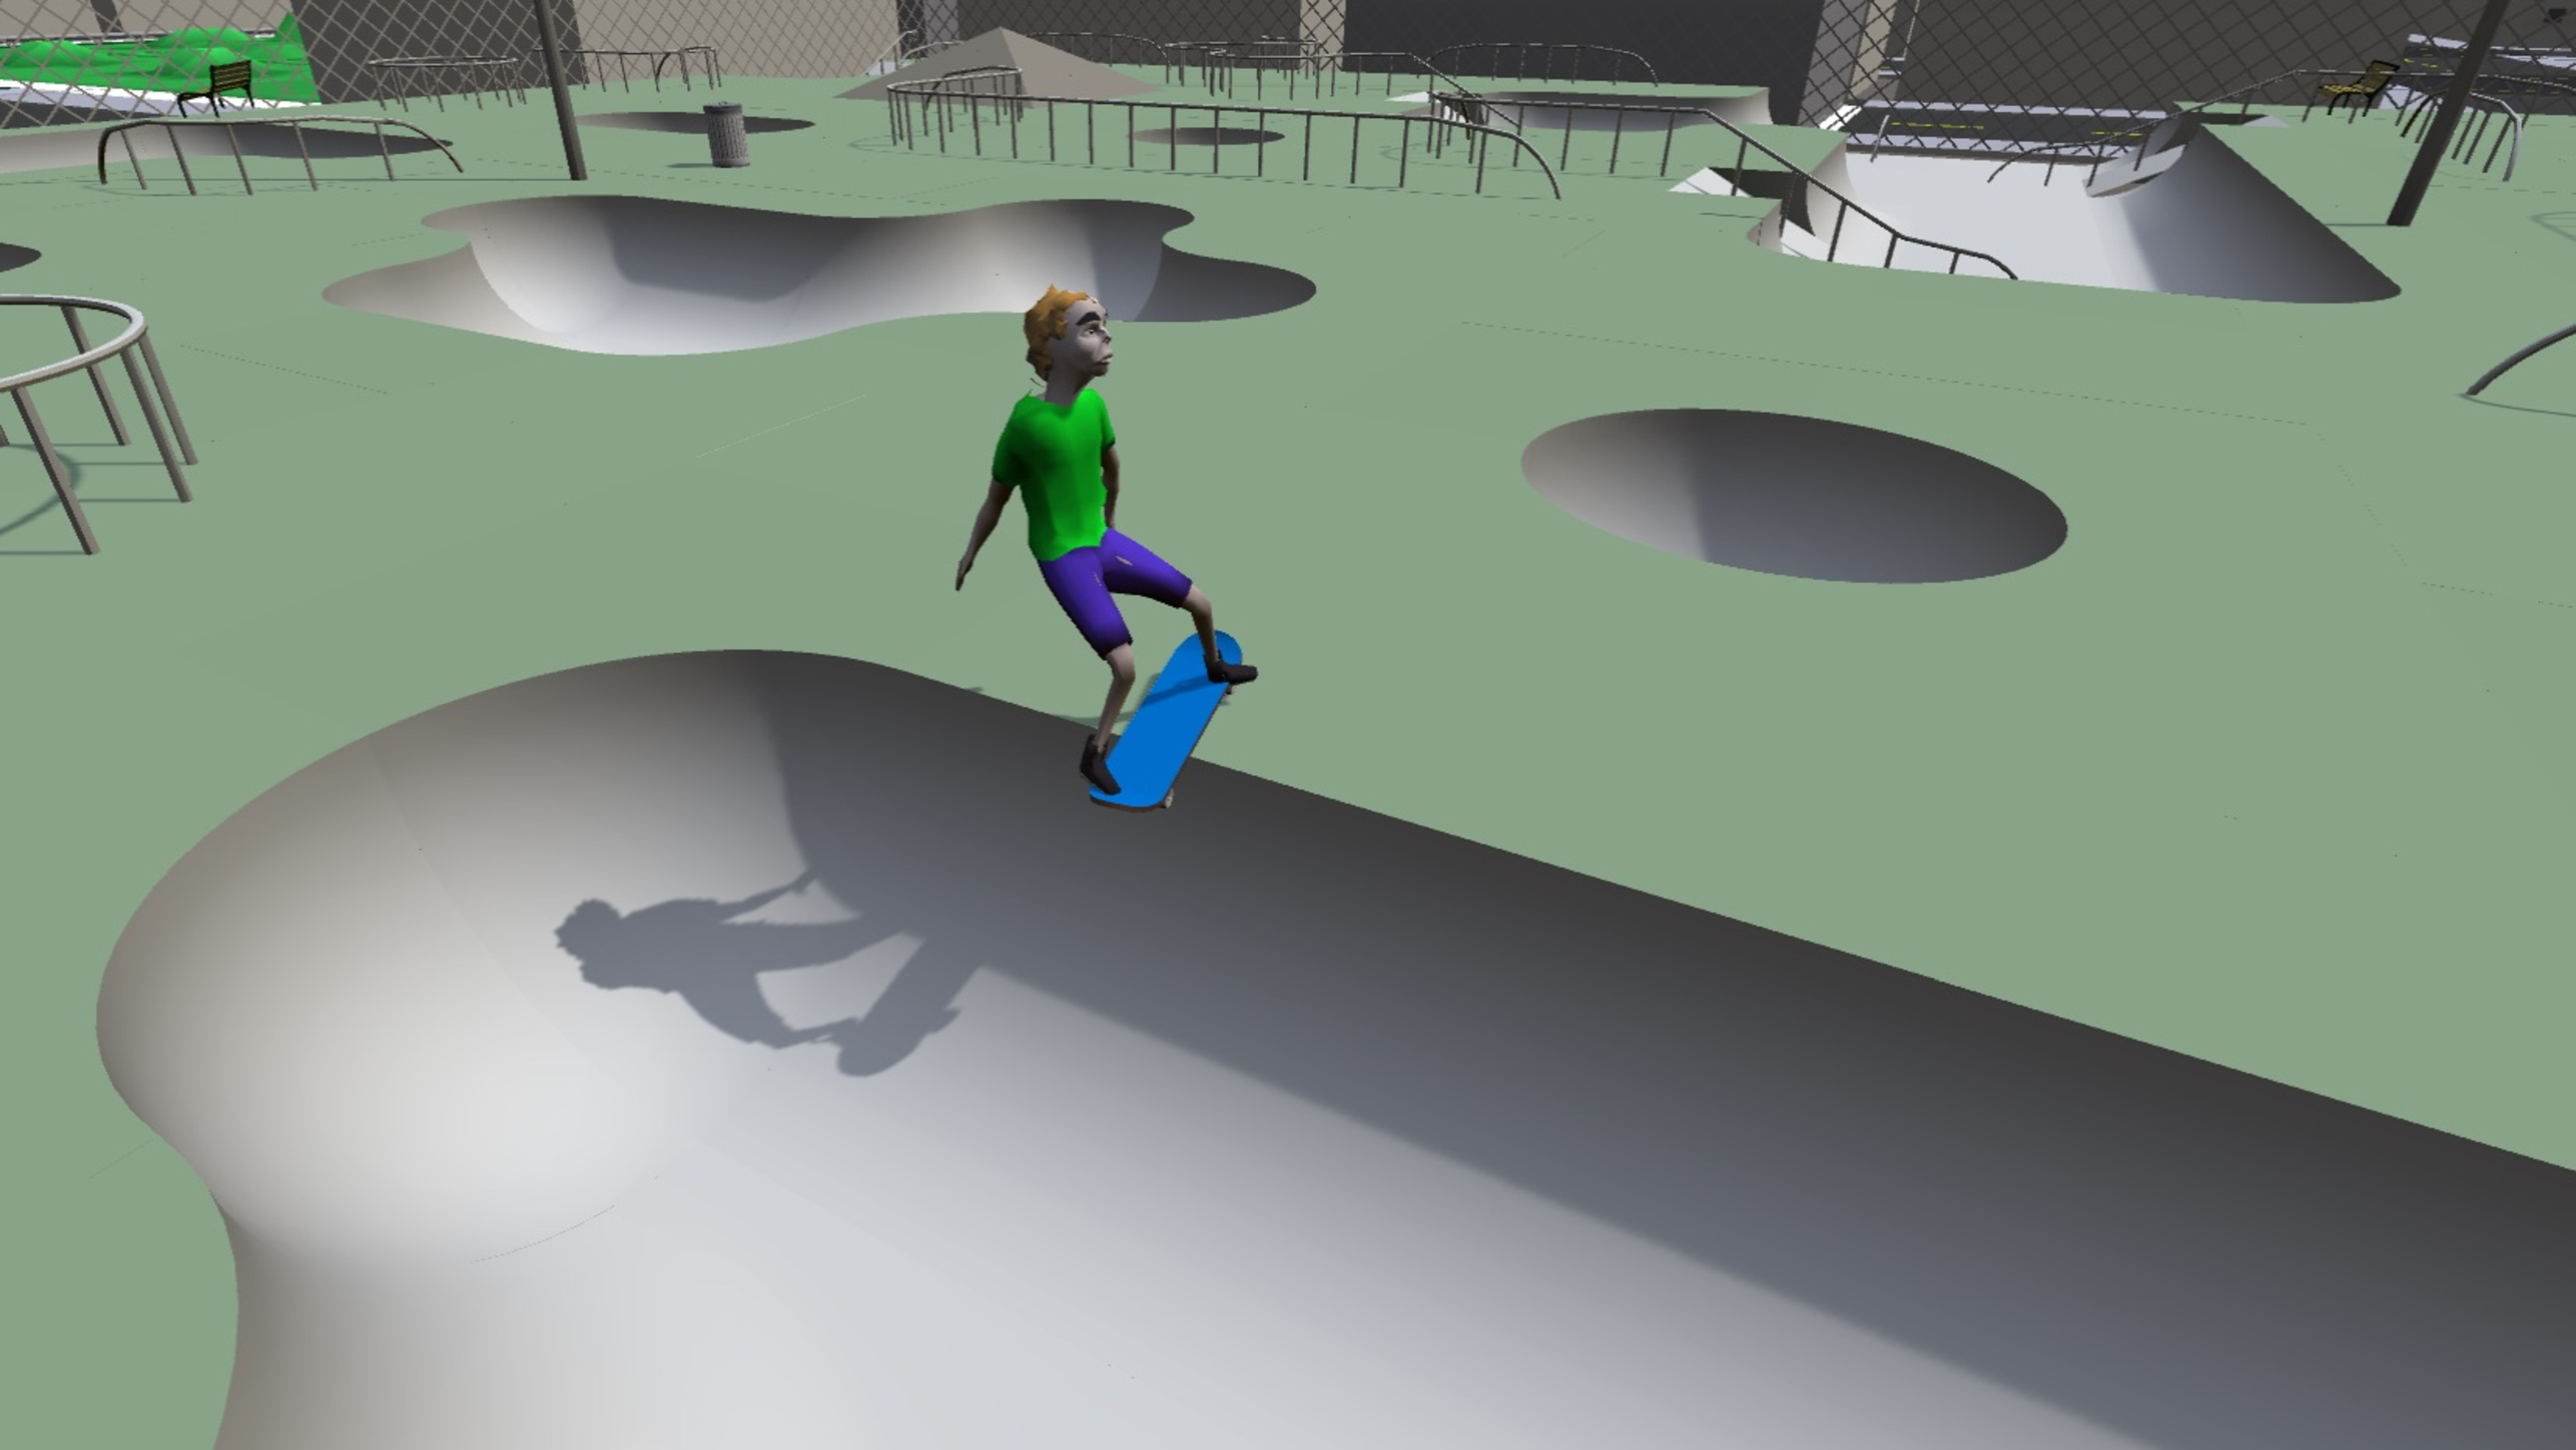
\includegraphics[width=\linewidth]{figures/soa/procSkater}
        \caption{\emph{Proc Skater 2016}~\citeonline{ParkerProcSkater}.}
        \label{fig:proc_skater}
    \end{subfigure}
    \hfill
    \begin{subfigure}[b]{0.48\linewidth}
        \centering
        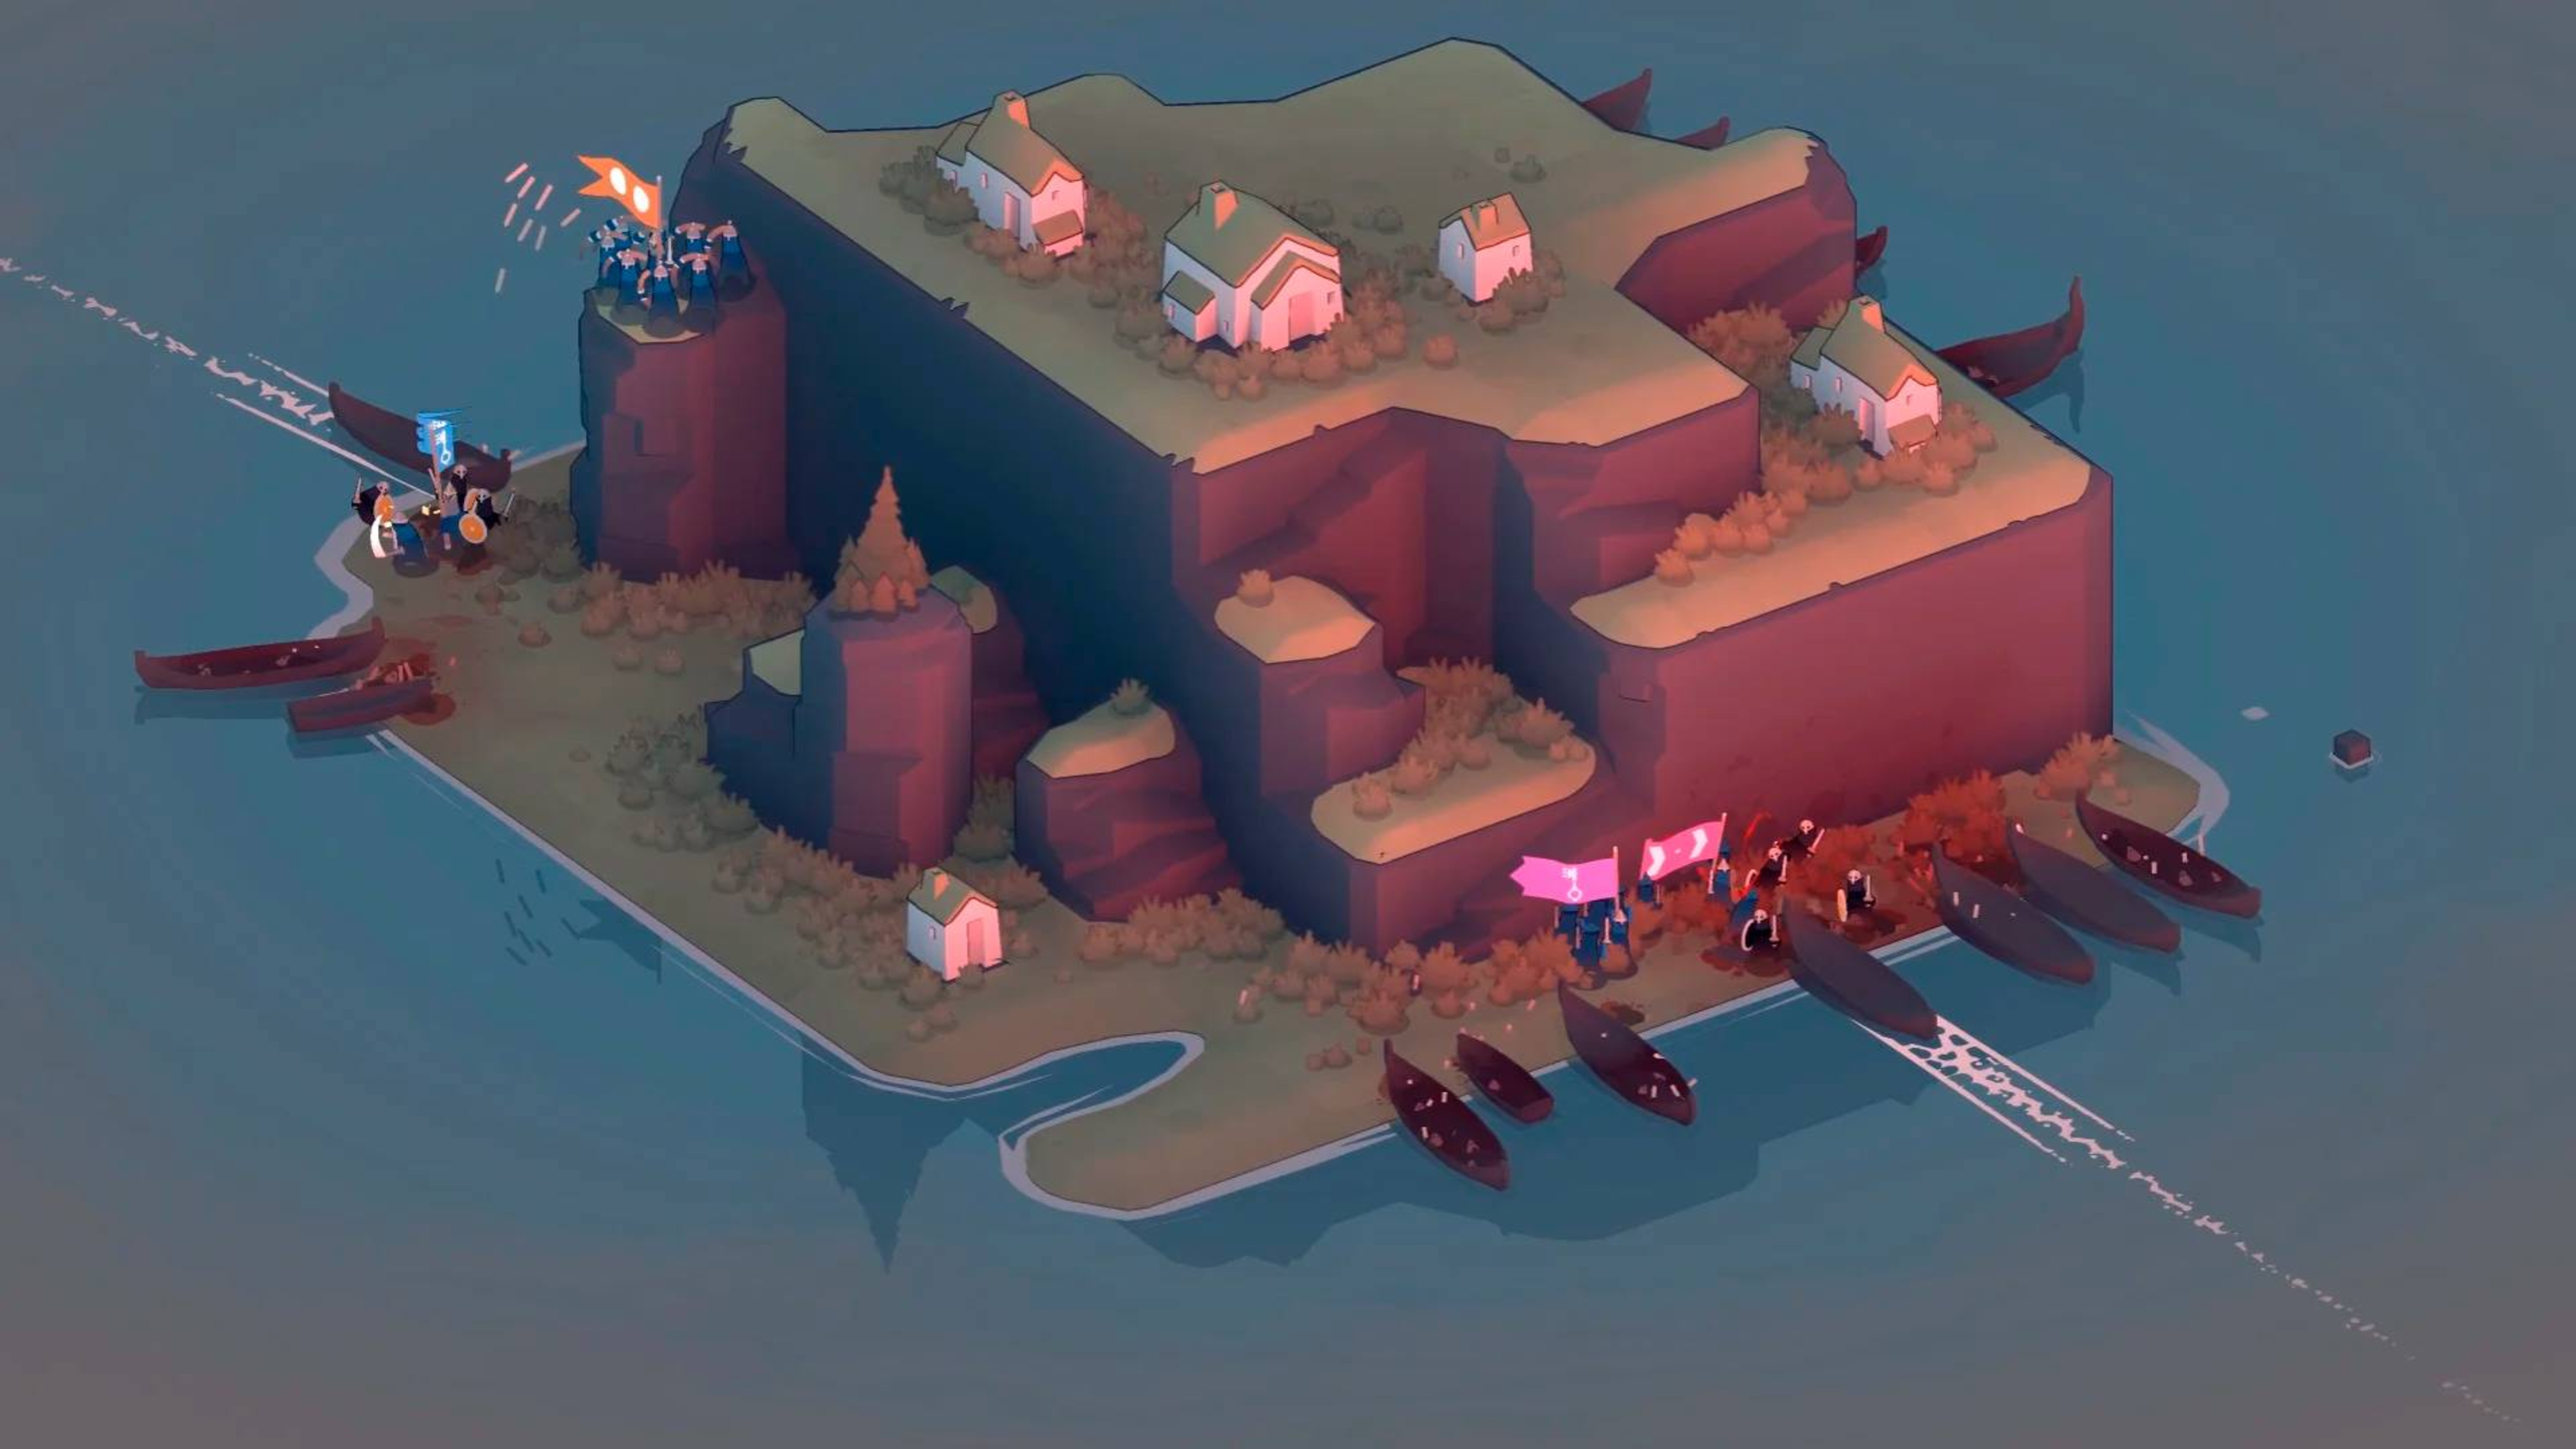
\includegraphics[width=\linewidth]{figures/soa/badNorth}
        \caption{\emph{Bad North}~\citeonline{StalbergBadNorth}.}
        \label{fig:bad_north}
    \end{subfigure}

    \vspace{0.5em}

    \begin{subfigure}[b]{0.48\linewidth}
        \centering
        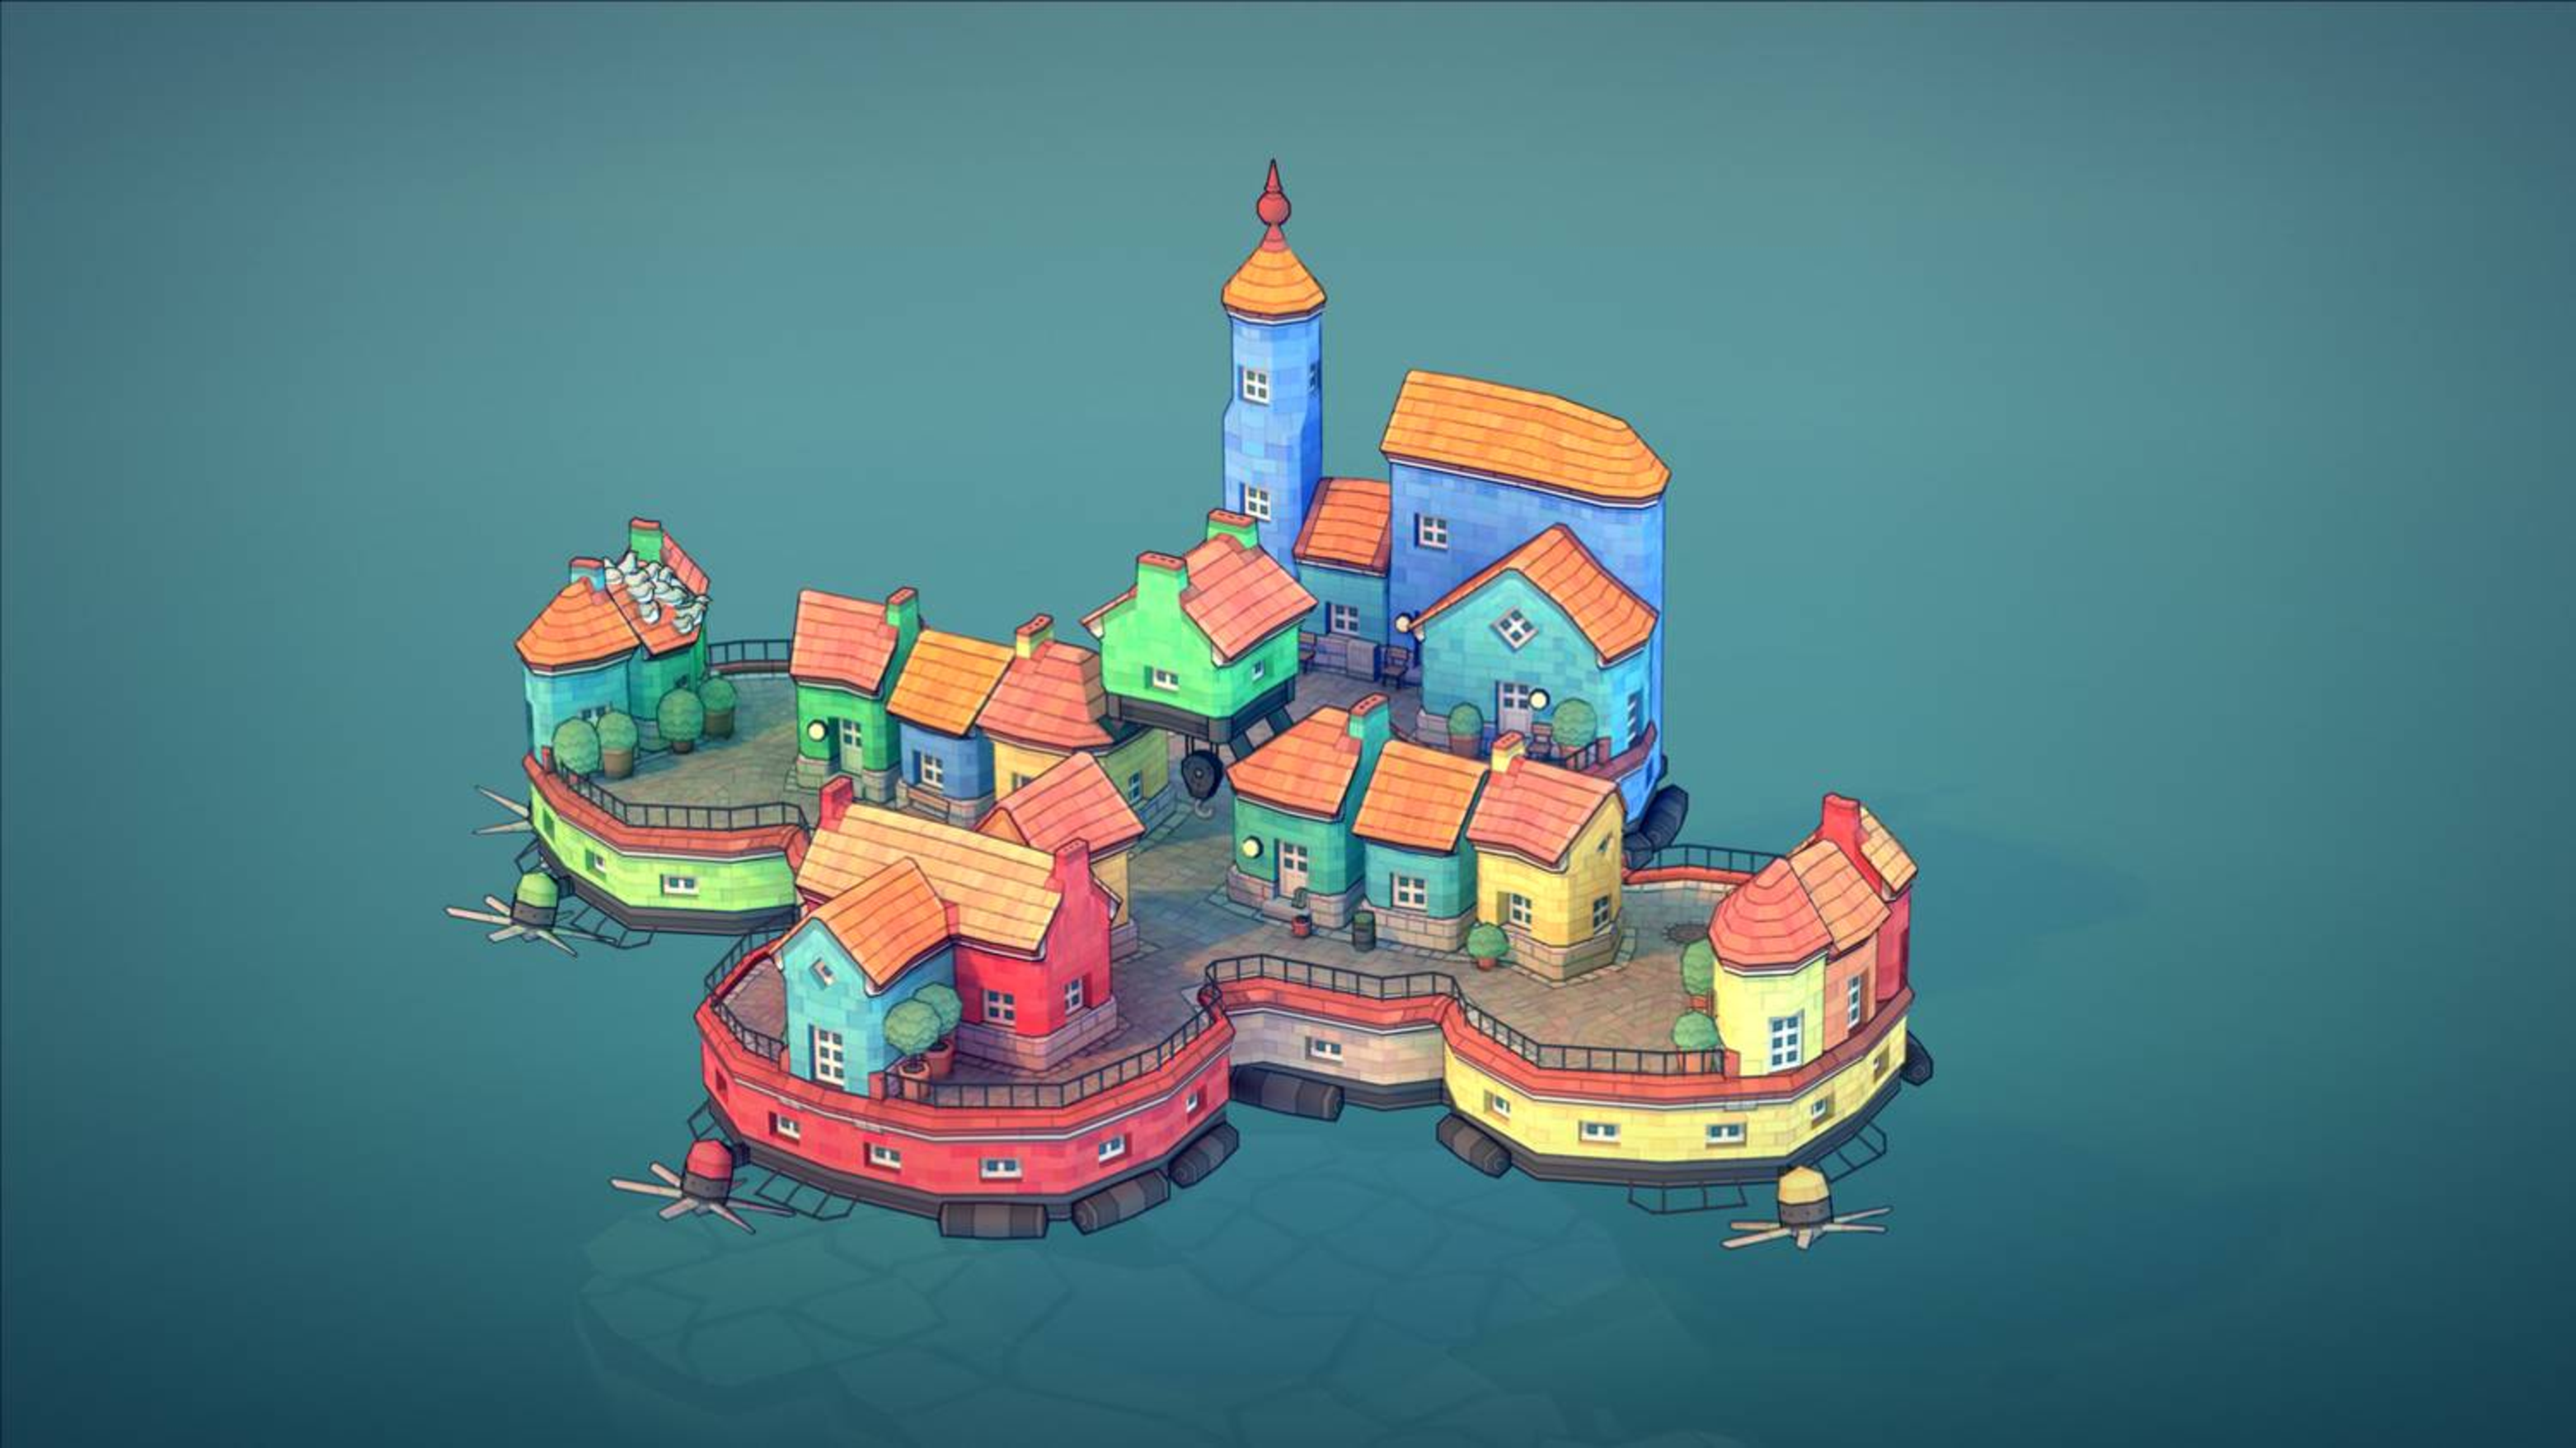
\includegraphics[width=\linewidth]{figures/soa/townsScaper}
        \caption{\emph{Townscaper}~\citeonline{StalbergTownscaper}.}
        \label{fig:townscaper}
    \end{subfigure}
    \hfill
    \begin{subfigure}[b]{0.48\linewidth}
        \centering
        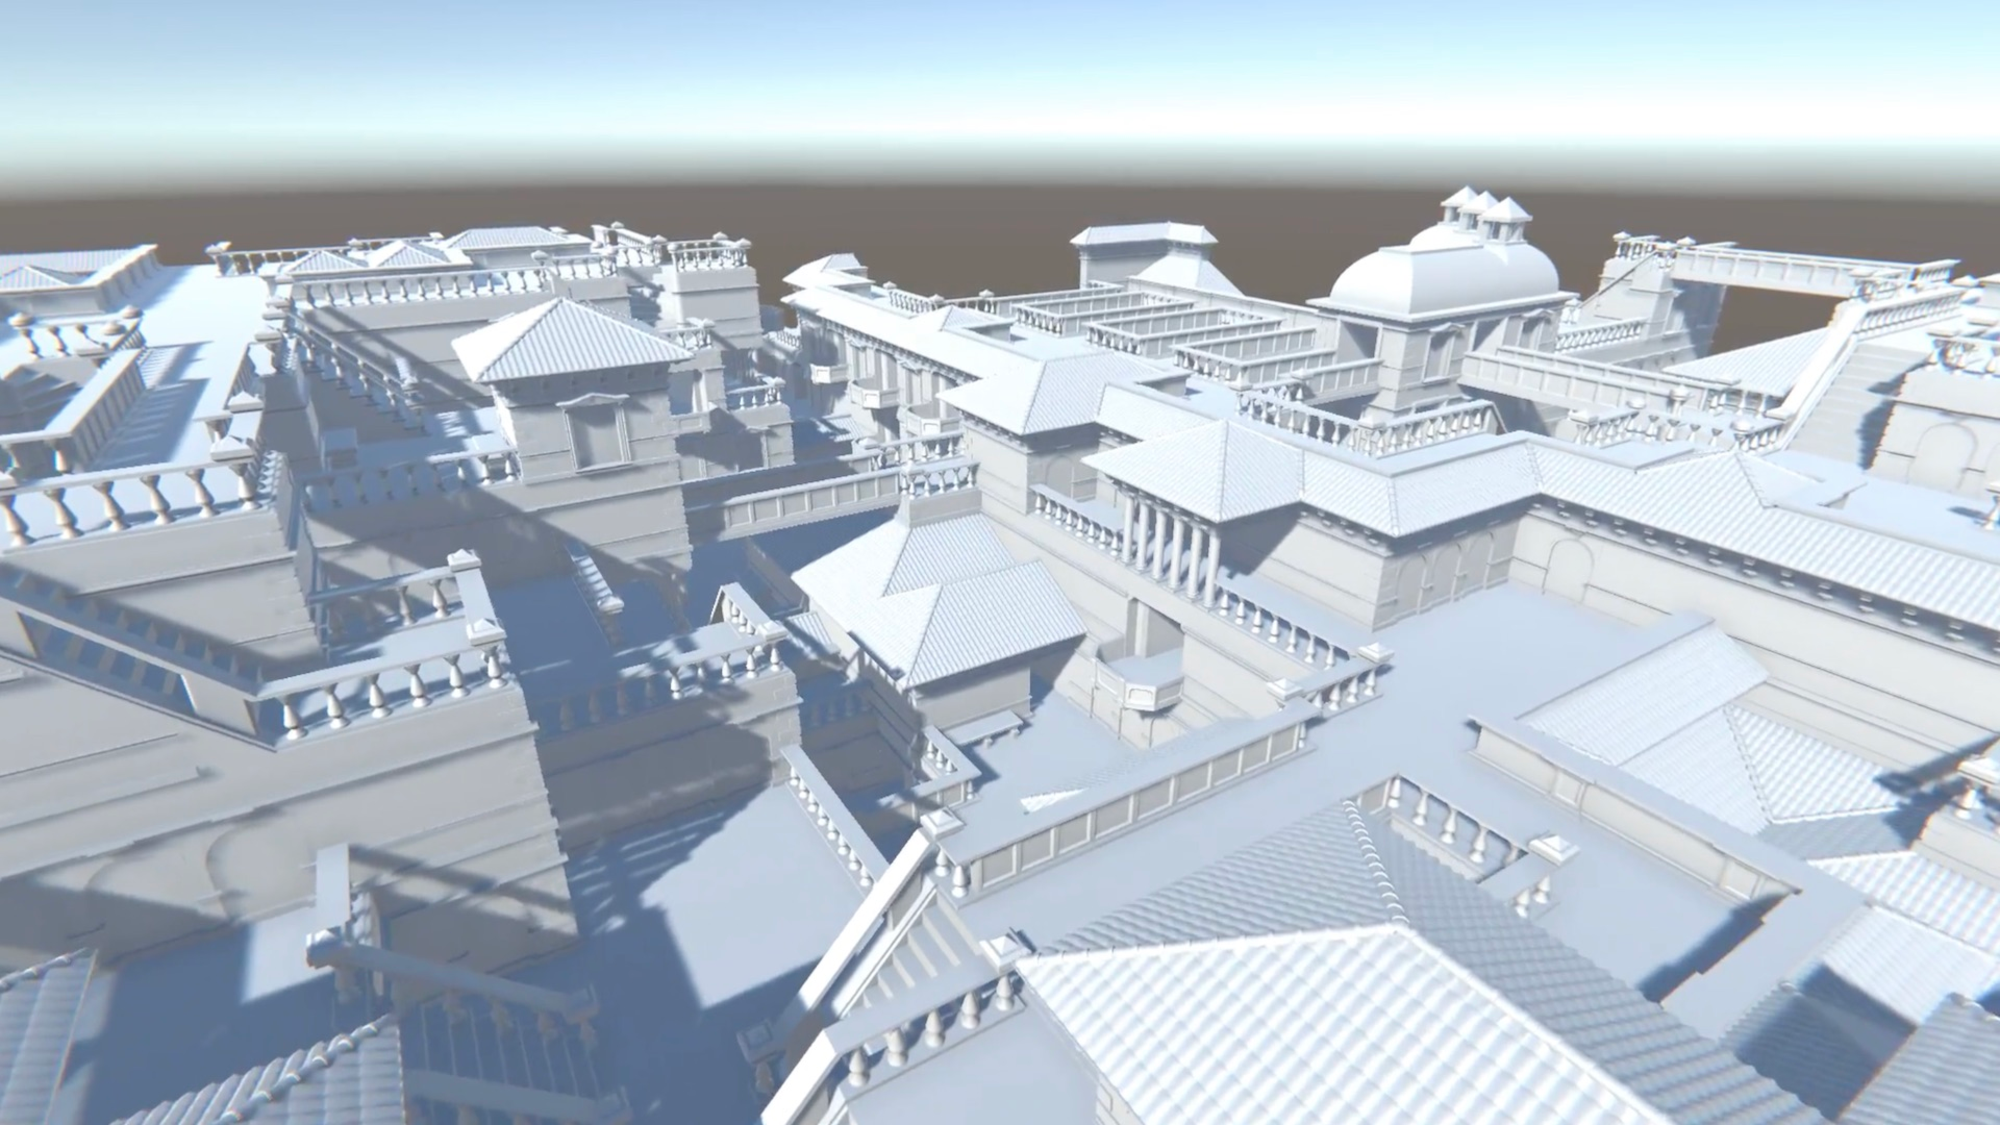
\includegraphics[width=\linewidth]{figures/soa/infiniteCity}
        \caption{\emph{Infinite City}~\citeonline{KleinebergInfiniteCity}.}
        \label{fig:infinite_city}
    \end{subfigure}

    \caption{Examples of WFC applications in game development.}
    \label{fig:wfc_game_development}

\end{figure}

\paragraph{Graph-based WFC.}

Original WFC operates on a square grid. Kim~\etal~\citebibliography{Kim2019a} extended WFC to graphs, allowing it to work with structures where nodes can have a different number of neighbors. They applied their graph-based WFC to problems such as Sudoku and the Voronoi graph 4-coloring problem, as shown in \figref{fig:graph_wfc}.

\begin{figure}[h]
    \centering
    \begin{subfigure}[b]{0.85\linewidth}
        \centering
        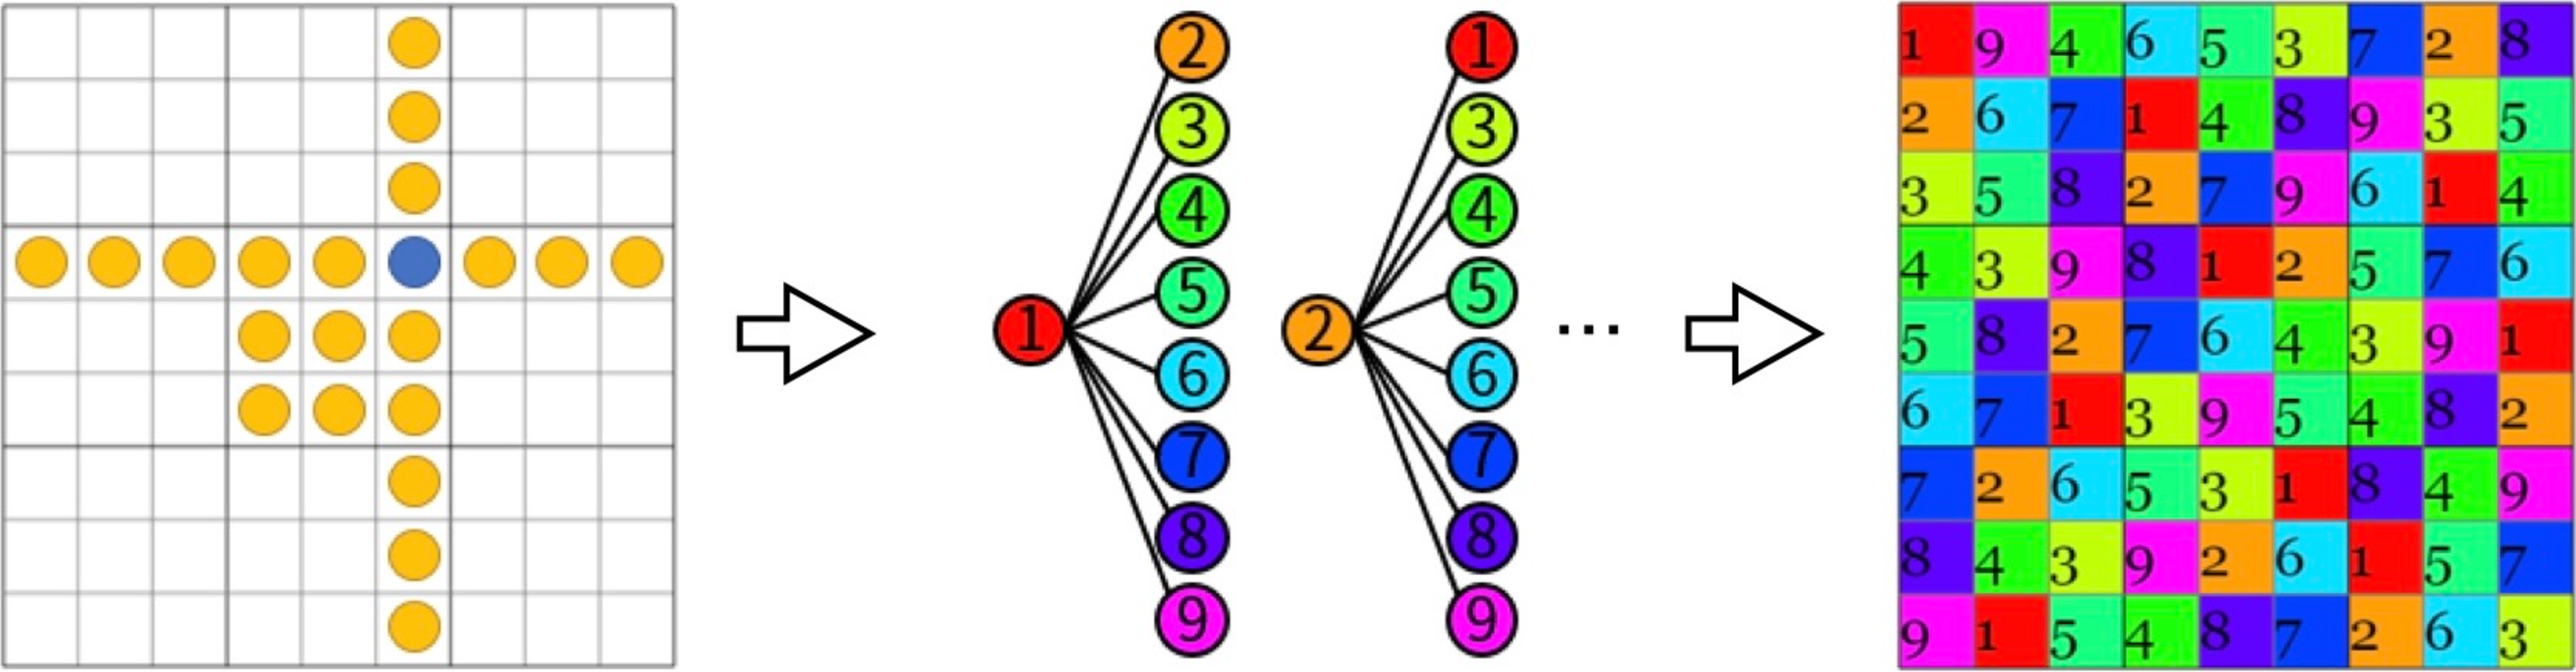
\includegraphics[width=\linewidth]{figures/soa/sudoku}
        \caption{Sudoku}
        \label{fig:sudoku}
    \end{subfigure}

    \begin{subfigure}[b]{0.85\linewidth}
        \centering
        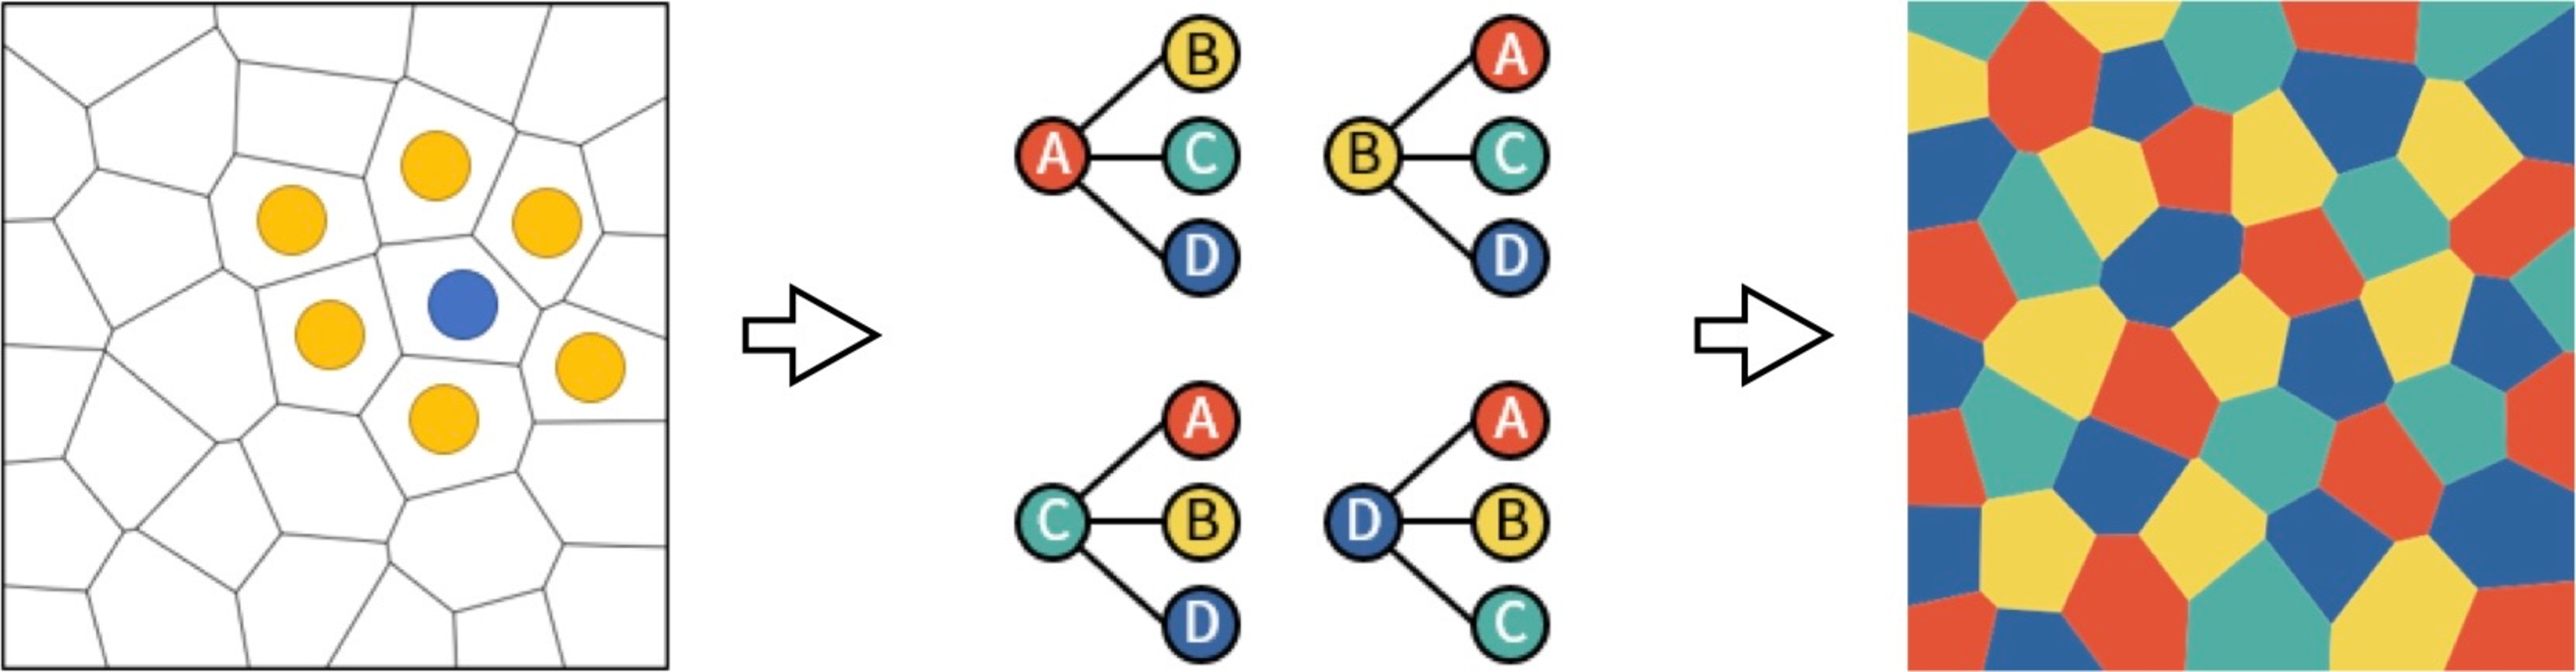
\includegraphics[width=\linewidth]{figures/soa/voronoi}
        \caption{Voronoi graph 4-coloring}
        \label{fig:voronoi}
    \end{subfigure}
    \caption[Graph-based WFC applications]{Examples of graph-based WFC applied to Sudoku and Voronoi graph 4-coloring~\citebibliography{Kim2019a}.}
    \label{fig:graph_wfc}
\end{figure}

Kim~\etal~\citebibliography{Kim2025a} later adapted this approach for procedural level generation in logic puzzle games. They applied WFC to \emph{Strimko} and \emph{Flow} puzzles, showing that it can generate levels that satisfy the constraints of these games faster than depth-first search and genetic algorithms.

\paragraph{Global Constraints.}

Standard Wave Function Collapse (WFC) relies on local neighbor rules, making it hard to control patterns across multiple cells or the entire map. Sandhu~\etal~\citebibliography{Sandh2019a} expanded WFC by adding non-local and design-level constraints, such as minimum and maximum item limits, tile dependencies, and changing weights dynamically during generation. These improvements allow the algorithm to follow global design requirements.

\paragraph{Designer Control.}

Langendam and Bidarra~\citebibliography{Lang2022a} focused instead on giving designers more direct control over the generation process. Their \emph{miWFC} introduces interactive tools for directly editing the output. A pencil tool allows users to select a cell and manually collapsing it to a tile, while a brush tool allows them to select areas to reset or preserve. Users can also define templates from an area of the output and place them multiple times in different locations or generations.

\paragraph{Scalability.}

Another limitation of standard WFC is the cost of generating large outputs. 
To fix this issue, Nie~\etal~\citebibliography{Nie2023a} introduced Nested Wave Function Collapse (\emph{N-WFC}), which splits a large map into a grid of smaller subgrids. Instead of solving the whole map at once, smaller WFC instances generate these subgrids step by step while matching edges with neighboring blocks. This reduces computation time from exponential to linear or polynomial, avoiding heavy backtracking and making it easy to create very large or infinite game worlds.

\paragraph{Non-Uniform Tiles.}

Standard WFC assumes that all tiles have the same size and shape. Piepenbrink and Bidarra~\citebibliography{Piep2025a} addressed this limitation with Non-Uniform Tile Wave Function Collapse (\emph{nutWFC}). Their approach allows tiles with different shapes and sizes to occupy multiple cells. To preserve the structure of these multi-cells tiles, they split each tile into single-cell units called \textit{atoms}, each identified by a unique ID. They then defined strict adjacency constraints between these atoms. These constraints ensure that all atoms of the same tile are collapsed together, preserving its original shape and size during generation.

\paragraph{Poetry.}

WFC has also been applied to less conventional domains. For example, O'Leary~\citeonline{OlearyPoetry} used WFC to generate poetry by treating syllables as tiles and defining constraints based on rhymes.

\end{document}